\documentclass{standalone}

\usepackage{tikz}
\usepackage{amsmath}
\usepackage{unicode-math}
\usepackage{xcolor}
\colorlet{darkRed}{red!40!black}
\colorlet{darkBlue}{cyan!50!black}
\colorlet{darkYellow}{yellow!50!black}


\begin{document}
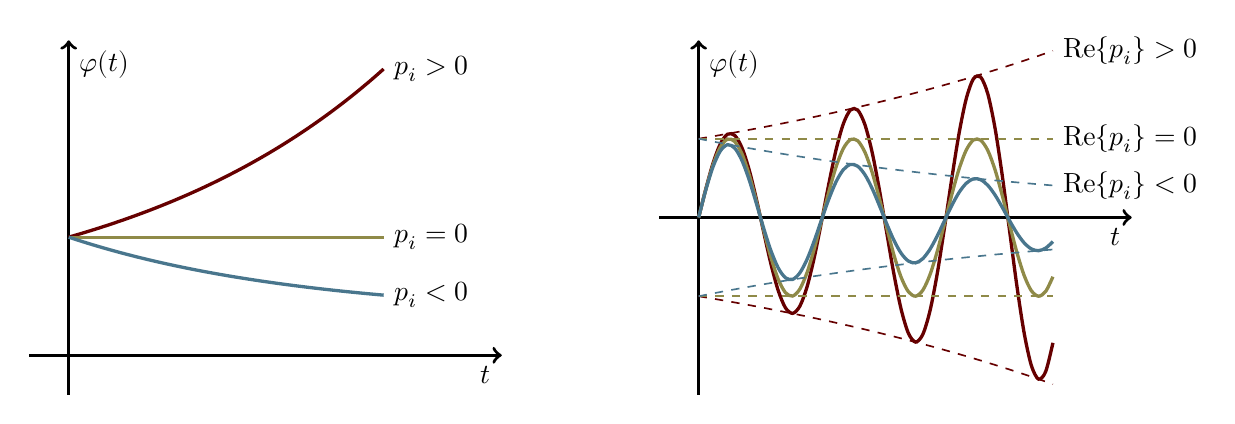
\begin{tikzpicture}[very thick]
  \draw[-to] (-0.5,0) -- ++(6.0,0) node[below left] {$t$};
  \draw[-to] (0,-0.5) -- ++(0,4.5) node[below right] {$\varphi(t)$};

  \draw[
    domain=0:4,
    smooth,
    variable=\x,
     draw =darkRed,
  ] plot ({\x}, {exp(\x / 3.5) + .5}) node[right] {$p_i > 0$};
  \draw[
    domain=0:4,
    smooth,
    variable=\x,
     draw =darkYellow,
  ] plot ({\x}, 1.5) node[right] {$p_i = 0$};
  \draw[
    domain=0:4,
    smooth,
    variable=\x,
     draw =darkBlue,
  ] plot ({\x}, {exp(-\x / 3) + .5}) node[right] {$p_i < 0$};

  \begin{scope}[xshift=8cm, yshift=1.75cm]
    \draw[-to] (-0.5,0) -- ++(6.0,0) node[below left] {$t$};
    \draw[-to] (0,-2.25) -- ++(0,4.5) node[below right] {$\varphi(t)$};

    \draw[
      domain=0:4.5,
      smooth,
      variable=\x,
       draw =darkRed,
      samples=50,
    ] plot ({\x}, {exp(\x / 6) * sin(deg(\x*4))});
    \draw[
      domain=0:4.5,
      smooth,
      variable=\x,
       draw =darkYellow,
      samples=50,
    ] plot ({\x}, {sin(deg(\x*4))});
    \draw[
      domain=0:4.5,
      smooth,
      variable=\x,
       draw =darkBlue,
      samples=50,
    ] plot ({\x}, {exp(-\x / 5) * sin(deg(\x*4))});

    \draw[domain=0:4.5, smooth, variable=\x, dashed, semithick, draw=darkRed]
    plot ({\x}, {exp(\x / 6)}) node[right] {$\mathrm{Re} \{ p_i \} > 0$}
    plot ({\x}, {-exp(\x / 6)});
    \draw[domain=0:4.5, smooth, variable=\x, dashed, semithick, draw=darkYellow]
    plot ({\x}, {1}) node[right] {$\mathrm{Re} \{ p_i \} = 0$}
    plot ({\x}, {-1});
    \draw[domain=0:4.5, smooth, variable=\x, dashed, semithick, draw=darkBlue]
    plot ({\x}, {exp(-\x / 5)}) node[right] {$\mathrm{Re} \{ p_i \} < 0$}
    plot ({\x}, {-exp(-\x / 5)});
  \end{scope}
\end{tikzpicture}
\end{document}
